\section{Test results}
 
kijjken kijken jajaja 18 180



\begin{figure}[!htb]
	\minipage{0.49\textwidth}
	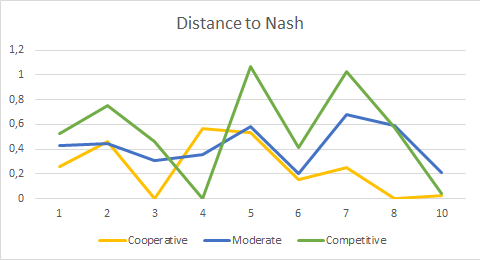
\includegraphics[width=\linewidth]{18_distance_nash}
	\caption{18 Rounds per Opponent}
	\label{fig:18_distance_nash}
	\endminipage\hfill
	\minipage{0.49\textwidth}
	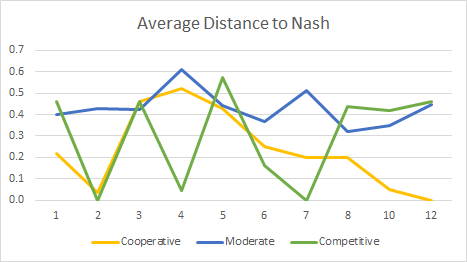
\includegraphics[width=\linewidth]{180_distance_nash}
	\caption{180 Rounds per Opponent}
	\label{fig:180_distance_nash}
	\endminipage\hfill
\end{figure}

%average distance to nash: cooperate   2 (180) lager
%						 competitive 2+7 (180) lager

%average distance to Pareto: cooperative 10 (18) hoger (domeinspecifiek, gaan we niks mee doen)

%we zien een correlatie tussen meer rounds en lagere agreements (stroevere tegenstander)

%average social welfare is gelijk voor beide

%2 competitive is langzaam

%onze utilities zijn altijd lager dan die van de tegenstander

%competitive utilities: 8 stijgt
%cooperative utilities: 4+5 stijgt
%moderate utilities: 4+5(+8) stijgt